\frame{\frametitle{Overshooting convection is characterized by a convective region mixing into a nominally stable region.}
	\begin{figure}[h]
		\centering
			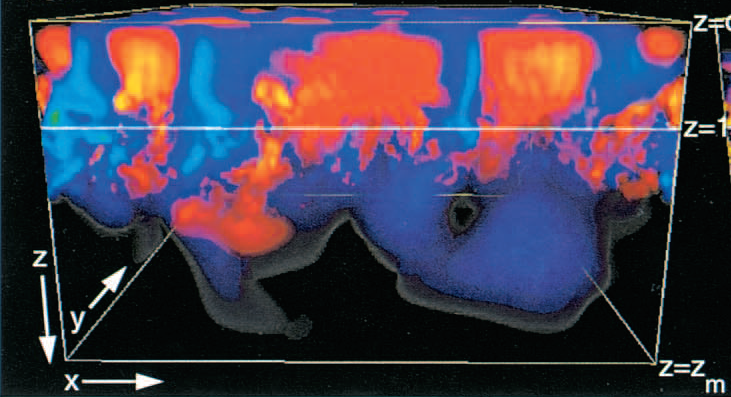
\includegraphics[width=.9\textwidth]{os_image.png}\footnote{\citep{Brummell2002}}
		\label{fig:figs_scdiagram}
	\end{figure}
}

\frame{\frametitle{This is distinct from penetrative convection, where the additional mixing extends the convection zone.}
	\begin{figure}[h]
		\centering
			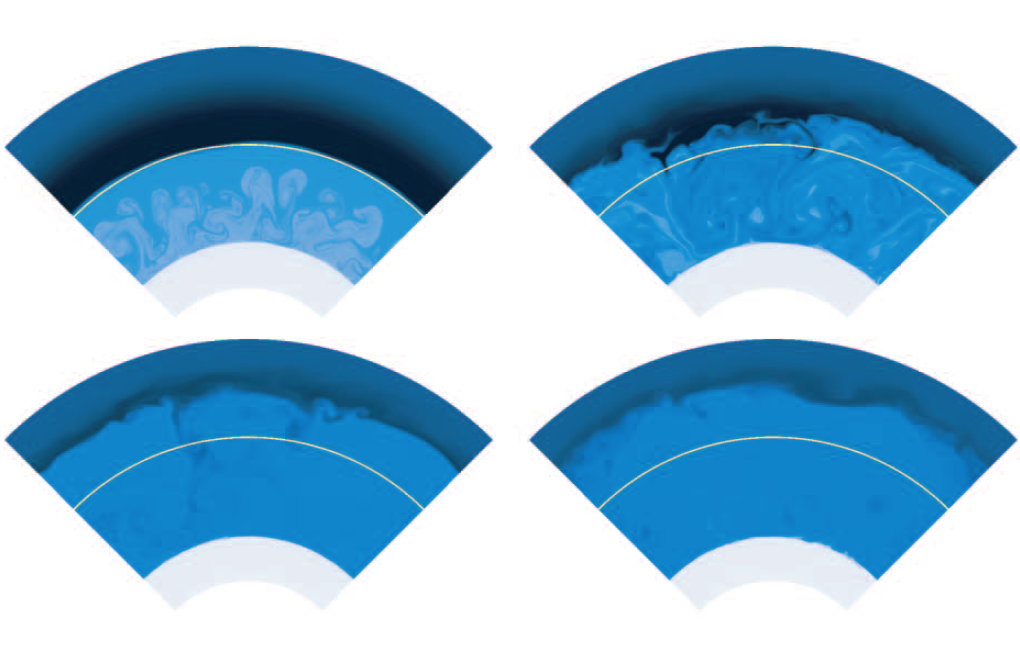
\includegraphics[width=.85\textwidth]{meakin_penetration.png}\footnote{\citep{Meakin2007}}
		\label{fig:figs_scdiagram}
	\end{figure}
}